\documentclass[11pt]{article}
\usepackage{fullpage}
\usepackage{graphicx}
\usepackage{float}
\usepackage{parskip}
\usepackage{natbib}

% Palatino for main text and math
\usepackage[osf,sc]{mathpazo}

% Helvetica for sans serif
% (scaled to match size of Palatino)
\usepackage[scaled=0.90]{helvet}

% Bera Mono for monospaced
% (scaled to match size of Palatino)
\usepackage[scaled=0.85]{beramono}

\newcommand{\blankline}{\quad\pagebreak[2]}

\newcommand{\R}{\mathbb R}

\usepackage[T1]{fontenc}
\usepackage{setspace}
\usepackage{multicol}
%\usepackage{indentfirst}
\usepackage{lastpage}
\usepackage{url}
%\pagestyle{fancy}
\usepackage{hyperref}
\usepackage{lastpage}
\usepackage{amsmath}
\usepackage{layout}

\renewcommand\labelitemi{--}

%\lhead{}
%\chead{}
%%%%%%%%%%%%%%%%%%%%%%%%%%%%%%%%%%%%%%%%%%%%%%%%%%%%%%%%%%%%%%

% Modify header here %%%%%%%%%%%%%%%%%%%%%%%%%%%%%%%%%%%%%%%%%
%\rhead{\footnotesize Text in header}

%%%%%%%%%%%%%%%%%%%%%%%%%%%%%%%%%%%%%%%%%%%%%%%%%%%%%%%%%%%%%%
%\lfoot{}
%\cfoot{\small \thepage/\pageref*{LastPage}}
%\rfoot{}

\usepackage{array, xcolor}
\usepackage{color,hyperref}
\hypersetup{colorlinks,breaklinks,linkcolor=red,urlcolor=red,anchorcolor=red,citecolor=black}

\bibliographystyle{agsm}
\bibpunct{(}{)}{;}{a}{}{,}

\title{Refinements}

\begin{document}

\maketitle

We are interested in comparing clusterings, and in particular in describing clusterings according to a tree structure.
We are particularly interested in this task for LDA, which has the additional complication that each sample (document) is not just assigned one cluster/topic, but is rather assigned a vector of weights corresponding to the fraction of that document that is in each cluster/topic.

The question addressed here will be whether given two clustering solutions, $\mathcal C_1$ and $\mathcal C_2$, if one of them can be interpreted as a refinement of the other.
Supposing that $\mathcal C_2$ has more clusters than $\mathcal C_1$, $\mathcal C_2$ being a refinement of $\mathcal C_2$ heuristically means that some of the clusters in $\mathcal C_1$ correspond more or less exactly to clusters in $\mathcal C_2$, and any cluster in $\mathcal C_1$ that doesn't correspond exactly to one cluster in $\mathcal C_2$ corresponds exactly to a union of clusters in $\mathcal C_2$.

It's a little bit silly to write this out formally, but we can make the following definitions for one cluster being a refinement of another and one clustering solution being a refinement of another clustering solution:

\begin{itemize}
\item A cluster $c_2$ is a refinement of another cluster $c_1$ if the samples comprising $c_2$ are a subset of the samples comprising $c_1$.

\item A clustering solution $\mathcal C_2$ is a refinement of a clustering solution $C_1$ if for every cluster $c_2 \in \mathcal C_2$, there exists $c_1\in \mathcal C_1$ such that $c_2$ is a refinement of $c_1$.
\end{itemize}

This idea works for the more standard clustering situation where each sample belongs to exactly one cluster.
However, it does not transfer over easily to the LDA situation where each sample has a weighted amount of ``belonging'' to each cluster.
We can try to make something work though.

\subsection*{Refinements for LDA}

Suppose that $C_1 \in \R^{n \times k_1}$, $C_2 \in \R^{n \times k_2}$ are the document by topic weight matrices for LDA solutions with $k_1$ and $k_2$ topics, respectively.
How do we adapt the refinement idea?
Well, if cluster $c_1$ in the first solution corresponds exactly to cluster $c_2$ in the second solution, then column $c_1$ of $C_1$ should be approximately the same as column $c_2$ of $C_2$.
Similarly, if cluster $c_1$ in the first solution ``split'' into clusters $c_2$ and $c_3$ in the second solution, then column $c_1$ of $C_1$ should be approximately equal to the sum of columns $c_2$ and $c_3$ in $C_2$.

We can express this idea in the following way: we require $C_1 = C_2 R$, where $R \in \{0,1\}^{k_2 \times k_1}$ is a matrix encoding a potential refinement structure for the clusters.
$R_{ij} = 1$ means that cluster $i$ in $C_2$ is a refinement of cluster $j$ in $C_1$.
We should require the row sums of $R$ to be 1 ($R \mathbf 1_{k_1} = \mathbf 1_{k_2}$), which indicates that each cluster in $C_2$ is a refinement of exactly one cluster in $C_1$.
The column sums of $R$ do not have to be 1, and the columns that have sum more than 1 correspond to clusters that have split into two or more new clusters.

Of course, we will almost never have an $R$ satisfying these conditions and also have exact equality of $C_1$ and $C_2 R$.
The best we can hope for is something approximate, and so we might want to find the matrix $R$ that makes $\|C_1 - C_2 R\|$ as small as possible.
Exhaustive search over all possible $R$ might be possible when we have small numbers of clusters, but an approximate or heuristic method will almost certainly be necessary with larger numbers of clusters.

\subsection*{Checking whether a refinement is more likely than chance}

We talked before about some ways of checking whether the quality of the refinement $\|C_1 - C_2 \hat R\|$, is better than we would expect if there were really no hierarchical structure.
Two possibilities we discussed were:
\begin{itemize}
\item Randomizing the rows of $C_2$ to get $C_2^*$, and recomputing the minimizing value of $\|C_1 - C_2^* R\|$, repeating this procedure many times and comparing the observed refinement quality to the randomized refinement quality.
\item Something similar, but instead of taking $C_2^*$ to be a row-permuted version of $C_2$, simulate data from the model implied by $C_1$, and compare the refinement quality in the simulations to that in the observed data.
\end{itemize}

On thinking about it a little more, I don't think this procedure is likely to work.
Both a split into two very distinct clusters and a split of a single cluster into two are going to give similar refinement matrices.
A potentially better approach follows.

The question: If we see a cluster split in two, how much do we ``believe'' in the split?
Are the daughters really distinct clusters, or are they an arbitrary splitting up of a single region of high density.

Proposed answer: Suppose cluster a splits into clusters b and c.
If this is a ``good'' split, then all the clusters that are refinements of a will also be refinements of b and c.
If it is not, not all oof the clusters that are refinements of a will also be refinements of b and c.
See the image below.

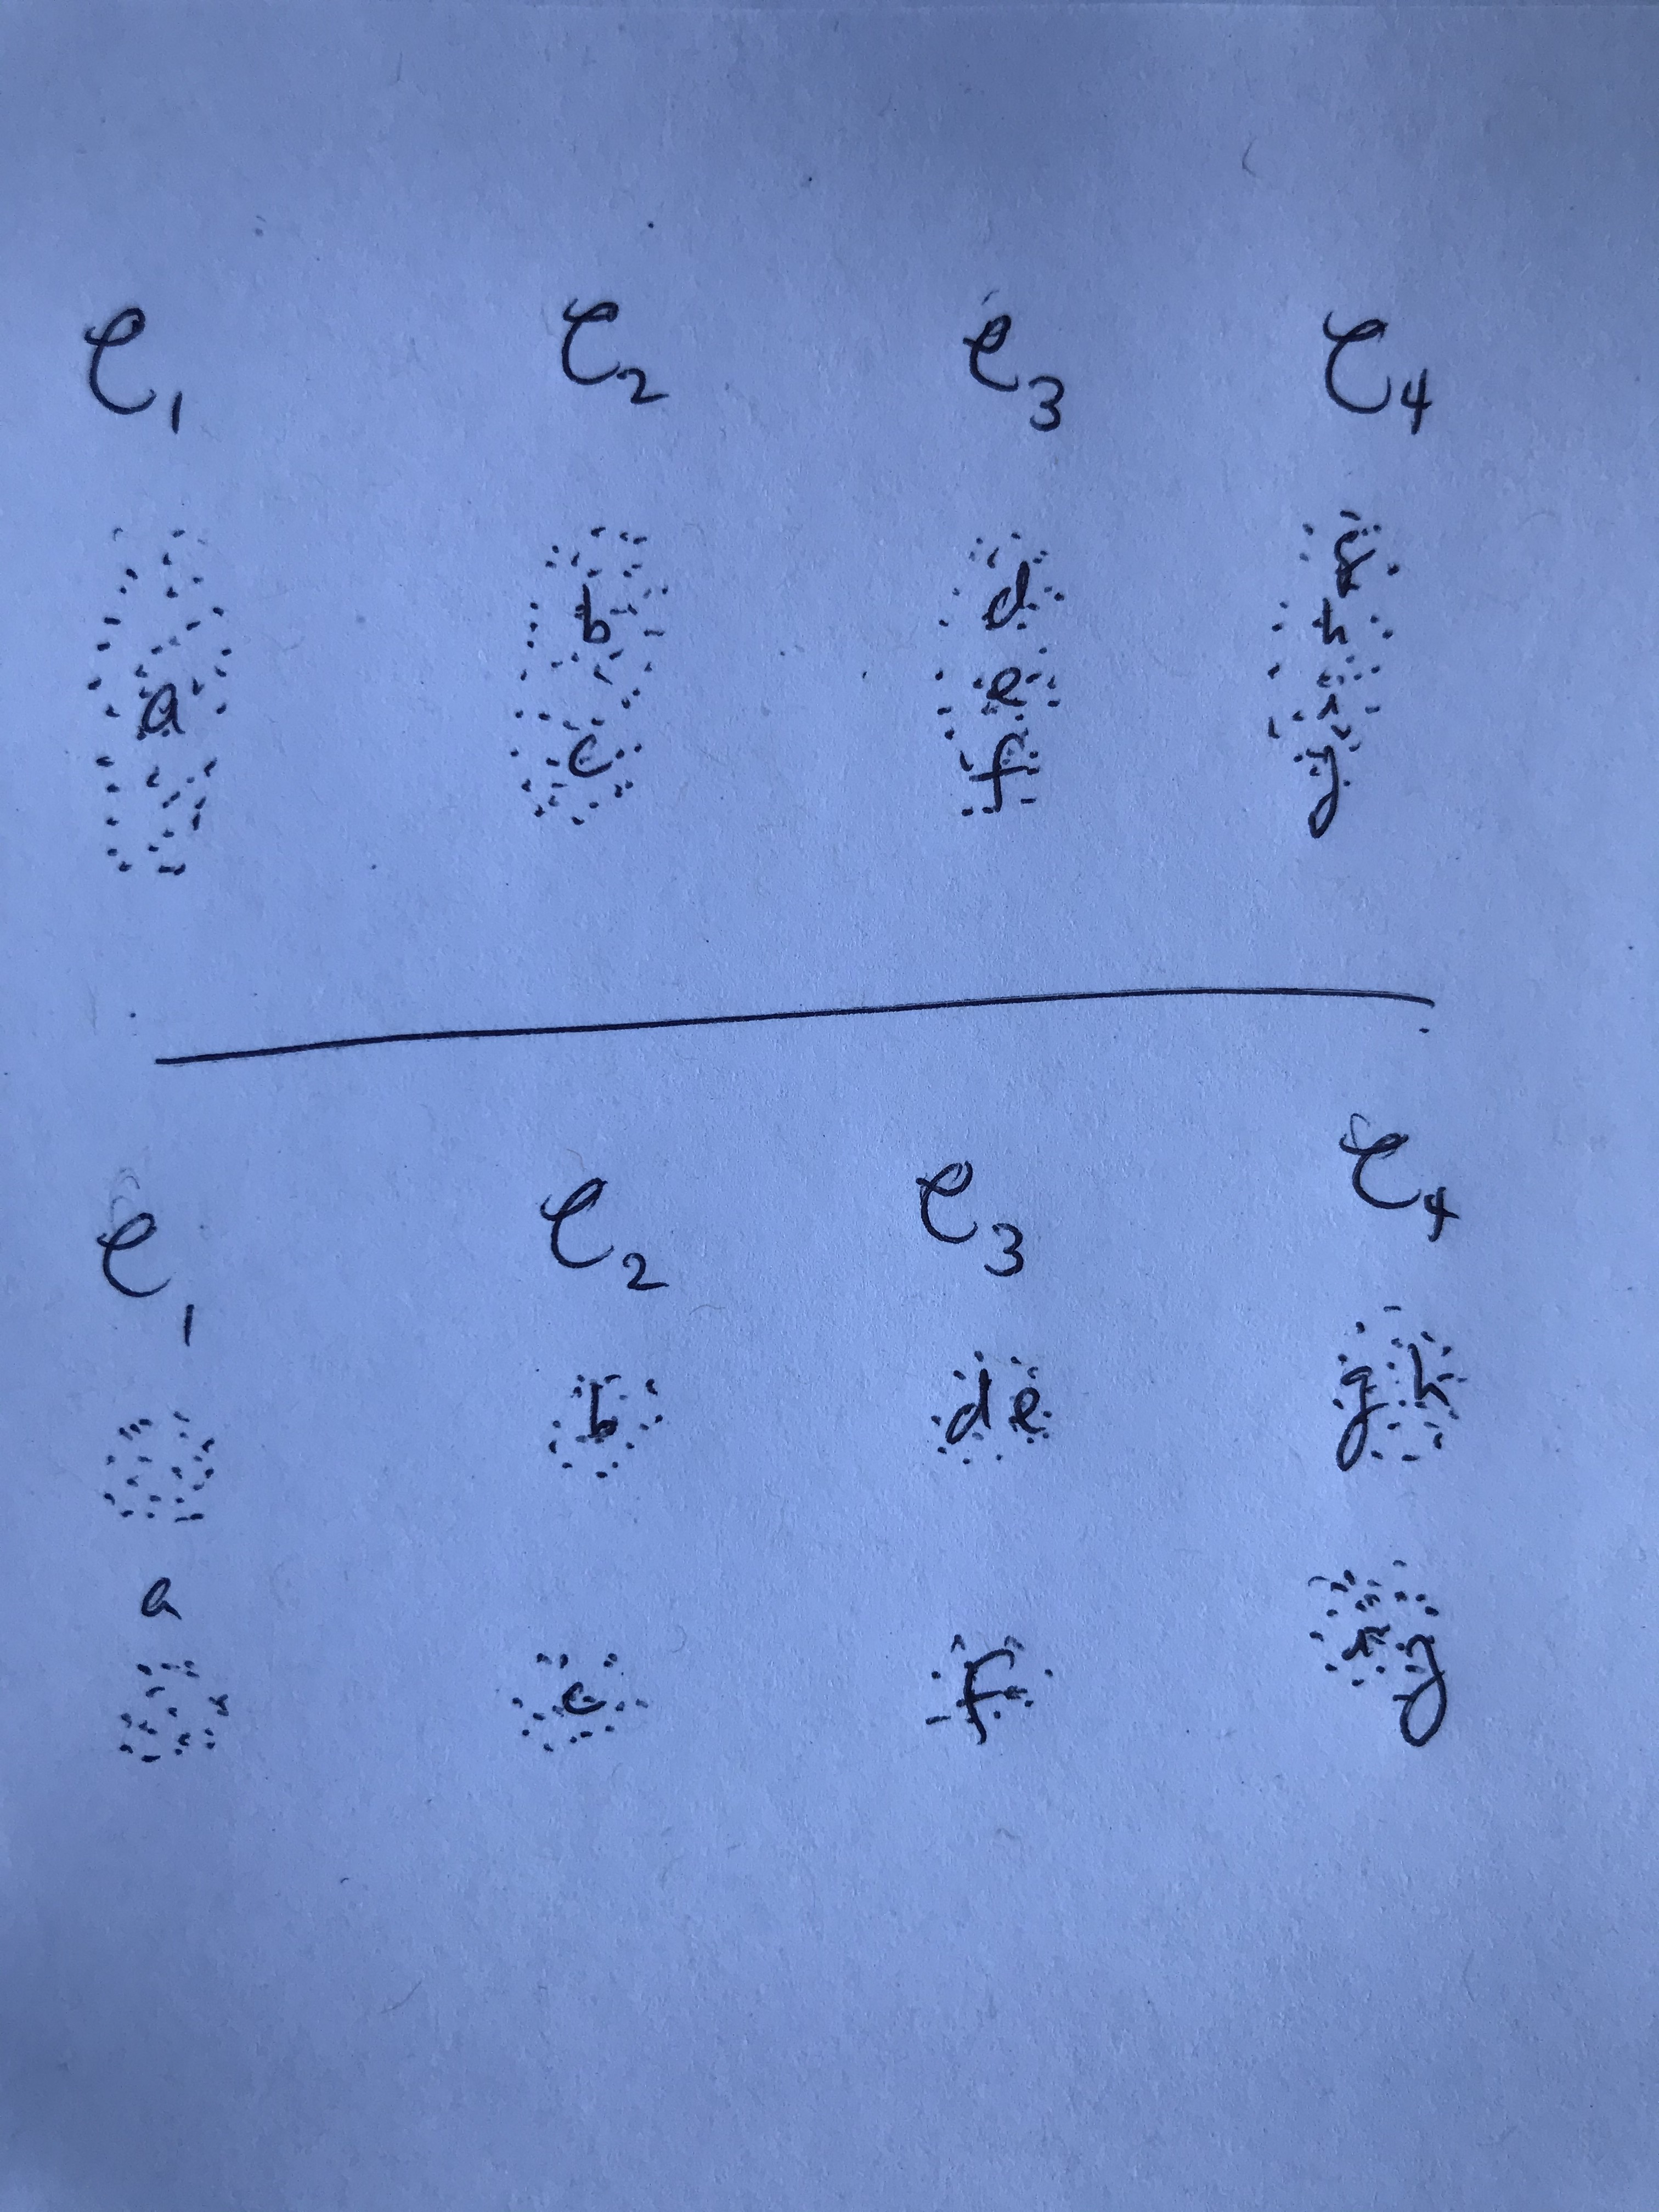
\includegraphics[width=.8\textwidth]{good-bad-split}

\end{document}
